\documentclass[UTF8]{ctexart}
\usepackage{amsmath}
\usepackage{diagbox}
\usepackage{textcomp}
\usepackage{graphicx}
\usepackage{float}
\usepackage{caption}
\usepackage{adjustbox}
\usepackage{subfigure}
\usepackage{geometry}
\usepackage{pifont}
\usepackage{gensymb}
\usepackage{bm}
\usepackage[colorlinks,linkcolor=blue]{hyperref}
\begin{document}
\renewcommand{\thefootnote}{\fnsymbol{footnote}}
\newgeometry{left=2cm,bottom=1cm,right=2cm}
\linespread{1.4}
\title{\vspace{-5em}\heiti弗兰克赫兹实验报告\vspace{-2.5em}}
\date{}
\maketitle
\begin{center}
{\fangsong 徐浩博\quad 软件02\quad2020010108}
\end{center}

\section{实验方法及实验数据}
\subsection*{1. 测试$I_P-U_a$曲线,根据曲线得到氩原子第一激发电位$U_g$}
连接好电路后,我们将实验条件设置为:灯丝电流$I_f=0.809A$,拒斥电压$U_R=6.992V$,第一栅极电压$U_G=1.500V$,将扫描电压的范围设置为$0-90V$,开启机器绘制$I_P-U_a$曲线,结果如下:
\vspace{-2em}
\begin{center}
\begin{figure}[H]
    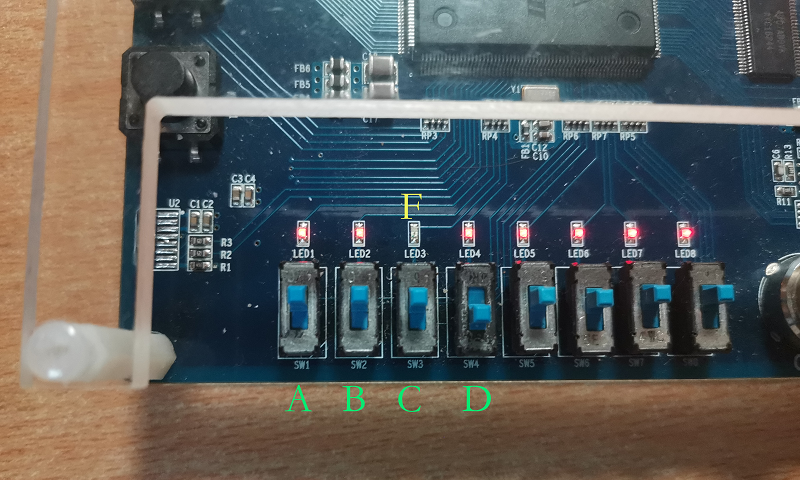
\includegraphics[scale=0.5]{1.png}\\
    \vspace{-3em}
    \centering{\caption{$I_P-U_a$曲线}}
\end{figure}
\end{center}
\vspace{-4em}
我们可以直观看出:\par
1. 随着$U_a$的增大,$I_p$按照一定频率波动:电子动能未达到基态氩原子跃迁到第一激发态的能量(设为$E_g$)时,因为量子力学规定氩原子的能量分立,因此电子只能与氩原子发生完全弹性碰撞,此时扫描电压升高,电子电流增大,$I_g$增大. 而当电子动能可以增加到$E_g$后,电子可以与氩原子碰撞使之跃迁,碰撞后电子动能减小$E_g$,故许多电子不能通过拒斥电场,从而$I_g$减小到谷底. 再增大$E_g$,碰撞后电子动能增大,$I_g$又逐渐增大;而电子动能达到$2E_g$时,电子可以使得两个原子跃迁,碰撞后动能又会大幅度减小,$I_g$又降到谷底. 如此循环往复,形成规律的波峰波谷. \par
2. 每个波动周期总体都比前一个周期$I_g$大:第一个波谷的产生是因为许多电子碰撞使一个氩原子跃迁产生的,而第二个波谷则是两次产生跃迁的碰撞,以此类推. 碰撞并跃迁是小概率事件:必须满足电子和原子取向、位置合适等一系列苛刻条件,故碰撞并跃迁的次数越大,概率越小;部分电子虽然动能足够,但可能并没有机会经历足量的碰撞,这部分电子贡献的电流使得$I_g$随$U_a$增大阶梯式上升.\\
考虑到波峰间的电位差事实上就代表了第一激发电位$U_g$,也即$E_g/e$,故可以通过线性拟合各波峰和对应的$U_a$值,获得$U_g$.
\vspace{-2em}
\begin{center}
    \begin{figure}[H]
        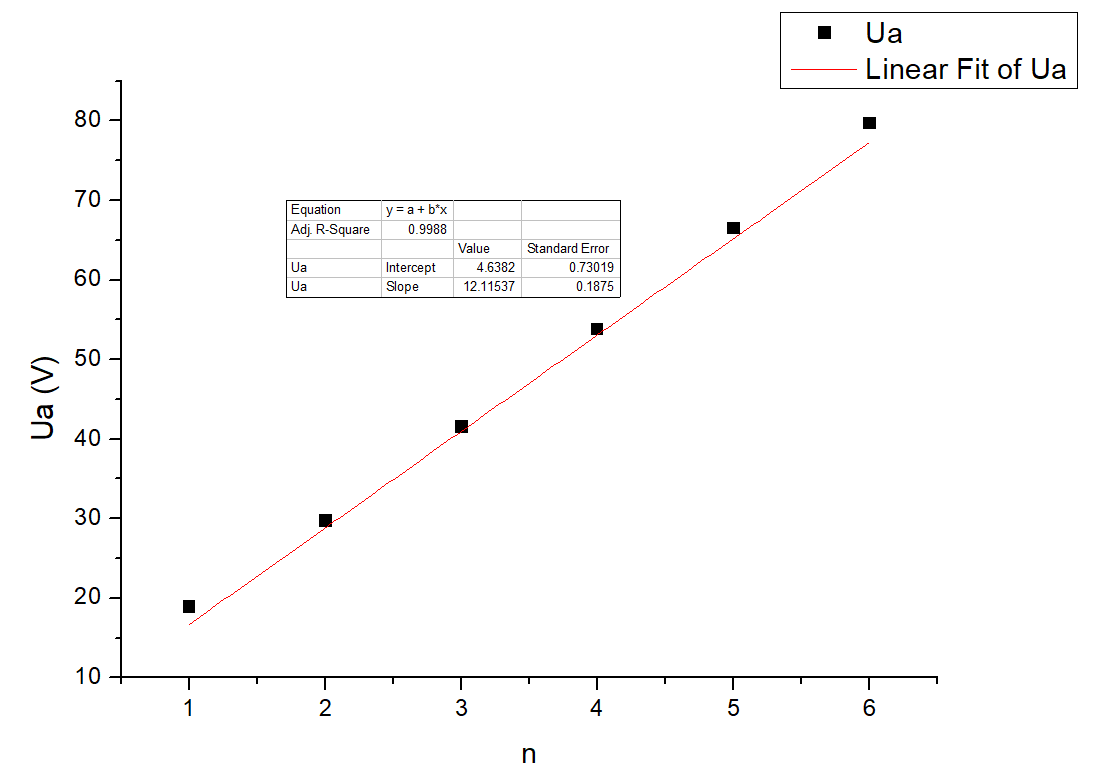
\includegraphics[scale=0.4]{linear.PNG}\\
        \vspace{-2.5em}
        \centering{\caption{第n级波峰和对应的$U_a$值拟合曲线}}
    \end{figure}
    \vspace{-1.5em}直线斜率$U_g=12.115V$ \quad
拟合系数$r=0.99952$
\end{center}
\begin{center}\end{center}
\vspace{-3em}
由拟合系数可以看出,拟合效果是不错的. 下面我们将计算$U_g$的不确定度:\par
A类不确定度:$\displaystyle{\frac{U_A}{b}=\sqrt{\frac{\frac{1}{r^2}-1}{n-2}}\quad \Longrightarrow\quad U_A=b\sqrt{\frac{\frac{1}{r^2}-1}{n-2}}=12.115\sqrt{\frac{\frac{1}{0.99952^2}-1}{6-2}}V=0.18V}$\par
B类不确定度:$\displaystyle{U_B=\Delta_{INS}=0.1\%b+0.01V=0.022V}$\par
$U_g$的不确定度:$\displaystyle{U_{U_g}\sqrt{U_A^2+U_B^2}=\sqrt{0.18^2+0.022^2}V=0.18V}$\\
故氩原子第一激发电位可表示为$U_g=(12.12\pm 0.18)V$.\par


\subsection*{2. 计算氩原子受激后回到基态辐射出的光波波长λ}
第一激发电位$U_g$与氩原子受激后回到基态辐射出的光波波长λ存在如下关系:\vspace{-1em}
\[eU_g=h\gamma=h\frac{c}{\lambda}\vspace{-1em}\]

故$\displaystyle{\lambda=\frac{hc}{eU_g}}=\frac{6.626\times2.998\times 10^8}{1.602\times 12.11}m=1.023\times 10^{-7}m$.
此光线在红外区域,故事实上很难看到氩光管发光. 由于红外线对眼睛等部位有危害,故需要用壳罩着管子防止对实验者身体造成损害.



\subsection*{3. 研究栅极电压$U_G$对$I_P$的影响}

保持灯丝电流$I_f=0.809A$,拒斥电压$U_R=7.000V$,将扫描电压的范围设置为$0-90V$,分别用机器描绘栅极电压$U_G=1.5V,\quad 2.0V,\quad 2.5V,\quad 3.0V,\quad 3.5V$时的$I_P-U_a$曲线,得到如下结果:\vspace{-2em}
\begin{center}
    \begin{figure}[H]
        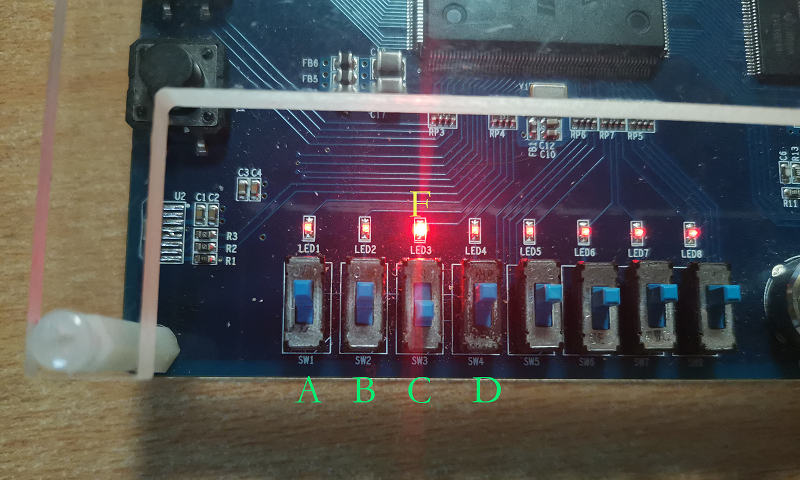
\includegraphics[scale=0.5]{2.png}\vspace{-3em}\\
        \centering{\caption{不同栅极电压下$I_P-U_a$曲线}}
    \end{figure}
\end{center}\vspace{-5em}
\paragraph{未归一化的曲线} 随着$U_G$的增大,$I_P$的峰值先增大(1.5V-2.0V)后减小(2.0V-3.5V)\par
解释:$U_G$增大产生的影响有1)消除空间电荷的影响,防止电子堆积,提高电子的发射效率,因此能够让更多电子进入后续电场,$I_P$升高;2)$U_G$过大时可能让电子能量在一定范围内上升,根据冉绍尔-汤森效应,有可能使得氩原子碰撞截面增大,从而增大了氩原子跃迁的可能,高动能电子数量减少,$I_P$降低;3)$U_G$过大使得电子在距离阴极更近处就拥有了发生非弹性碰撞的动能,因此可以发生非弹性碰撞的路程更长,发生非弹性碰撞次数的数学期望升高,$I_P$降低.\par
综合以上原因,$U_G$增大,1)因素使得$I_P$增大,2)、3)因素使得$I_P$减小. 在$U_G$较小时,1)为主要影响因素;较大时,2)、3)为主要影响因素;最终表示成随着$U_G$的增大,$I_P$的峰值先增大后减小.\vspace{-1em}
\paragraph{归一化的曲线} 峰值对应的$U_G$接近\par
解释:峰值对应的$U_G$接近,是因为总体上使得电子加速的总能量只与扫描电压有关,与栅极电压无关;而电子加速的总能量到达n倍的激发能量,就显示峰值. 因此,峰值的出现与扫描电压关系更大.

\subsection*{4. 研究栅极电压$U_R$对$I_P$的影响}

保持灯丝电流$I_f=0.809A$,栅极电压$U_G=1.500V$,将扫描电压的范围设置为$0-90V$,分别用机器描绘拒斥电压$U_R=5.0V,\quad 6.0V,\quad 7.0V,\quad 8.0V,\quad 9.0V$时的$I_P-U_a$曲线,得到如下结果:\vspace{-2em}
\begin{center}
    \begin{figure}[H]
        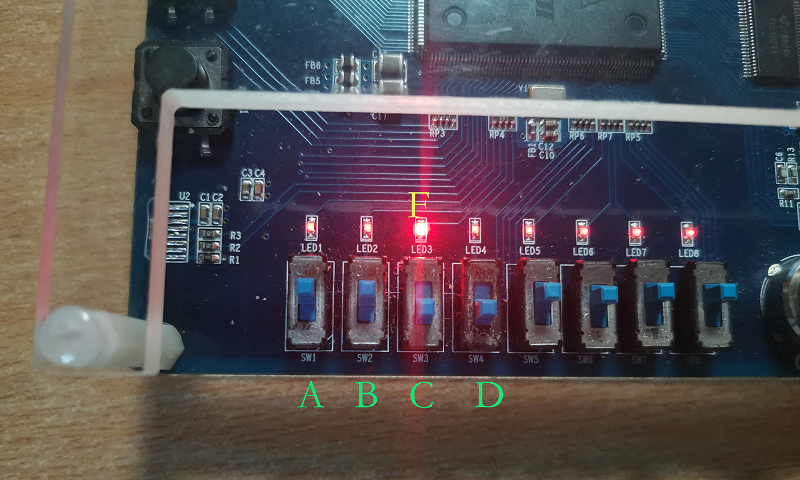
\includegraphics[scale=0.6]{3.png}\\\vspace{-3em}
        \centering{\caption{不同拒斥电压下$I_P-U_a$曲线}}
    \end{figure}
\end{center}
\vspace{-5em}
\paragraph{未归一化的曲线} 随着$U_R$的增大,$I_P$的峰值减小\par
解释:拒斥电压增大,低动能的电子无法穿过拒斥电场,故$I_P$电流减小.
\paragraph{归一化的曲线} 随着$U_R$的增大,$I_P$的峰值右移\par
解释:拒斥电压增大,无法通过拒斥电场的低动能电子可能会积聚在扫描电压和拒斥电压交界处,形成一个排斥电场,故扫描电压需要更大,才能保证电子具有发生足够次数非弹性碰撞的动能. 所以每个峰值对应的$U_a$会增大,峰值右移.

\subsection*{5. 研究和测量氩原子更高激发态的$I_P-U_a$曲线}
下面我们连接高激发态电路并完成实验,在拒斥电压分别为2.0V, 2.5V, 3.0V的条件下改变扫描电压,绘制$I_P-U_a$曲线.\vspace{-1em}
\begin{center}
    \begin{figure}[H]
        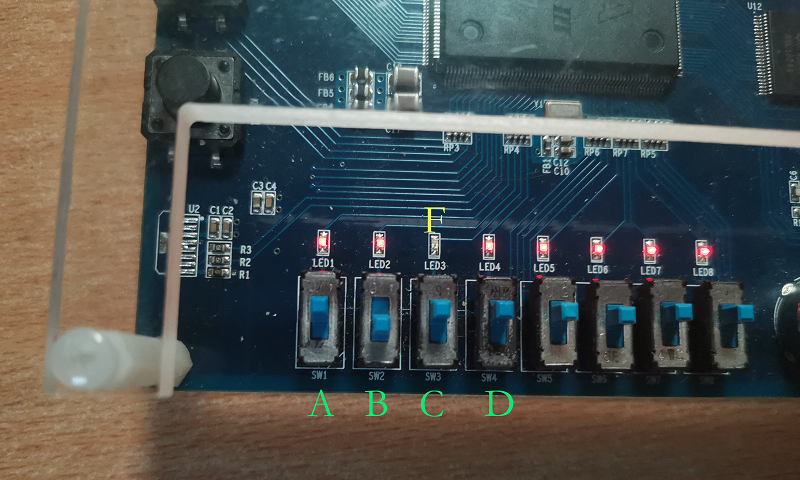
\includegraphics[scale=0.5]{4.png}\\\vspace{-3em}
        \centering{\caption{$I_P-U_a$曲线}}
    \end{figure}
\end{center}\vspace{-3em}
可以明显看出,整个曲线呈两个阶梯状,且似有周期性变化. 我们选取拒斥电压为3.0V的图线研究,四个极大值点分别在$U_a$取$U_{a1}=6.78V$,$U_{a2}=12.75V$,$U_{a3}=19.14V$,$U_{a4}=24.66V$时取到,下面我们就这一条曲线来分析:
氩原子的第一电离能约为$15.760V$\footnote{详见参考文献.\label{ft}},那么在高能的情况下,氩原子很可能发生了电离,生成Ar(I)离子. 我们考察Ar光谱表,发现强度较大的几条线分别为$1048.21987Å, 723.3606Å, 671.8513Å$\textsuperscript{\ref {ft}},其中前者为Ar原子跃迁,后两者为Ar(I)离子跃迁;由于后两者波长相近,考虑到仪器精度可能不足以分辨,故可以平均为一条$\lambda=697.6060Å$的谱线. 因此,两条跃迁谱线对应的电位分别为$U_1=11.83V, U_2=17.77V$. 若$U_{a1}=6.78V$对应激发电位为$U_1=11.83V$的谱线,那么$U_{a2}=U_{a1}+5.97V$大致与$U_2=U_1+5.94V$的谱线对应. 可以看到$5.97V$与$5.94V$相差极小,吻合得是很好的. 而$U_{a3}\approx U_{a1}+U_1$,$U_{a4}\approx U_{a1}+U_{2}$,故可以归结为
\begin{table}[H]
    \begin{center}
        \begin{tabular}{|c|c|c|c|c|}
            \hline
            极大值点对应电位&$U_{a1}$&$U_{a2}$&$U_{a3}$&$U_{a4}$\\
            \hline
            实际值/V&6.78&12.75&19.14&24.66\\
            \hline
            预测原因&谱线1&谱线2&谱线1+谱线1&谱线1+谱线2\\
            \hline
            预测值/V&6.78&12.72&18.61&24.55\\
            \hline
        \end{tabular}
    \end{center}
\end{table}\vspace{-2em}
可以看出,在$U_a$测量点间隔大约为$0.2V$的前提下,预测值和理论值还能很好的吻合,证明了我们的理论有一定的正确性. 至于曲线前两个峰值、后两个峰值之间的平台,我们认为这是由于Ar和Ar(I)向更高能级跃迁,跃迁能量较小而近似可以看作为连续谱的结果.

\section{思考题}
\subsection*{1. 为什么$I_P-U_a$呈周期性变化}
开始时,扫描电压升高,板极电流也升高;当扫描电压升高到大于氩原子第一激发电位时,就可以产生非弹性碰撞了. 发生碰撞的电子动能会减小,因此能够穿越拒斥电场的电子数减小,板极电流减小. 中间的转折点就是峰值. 之后随着$U_a$的上升,1)达到激发电位的n倍的路程越来越短,因此有更多几率引发第n次跃迁,电流减小,2)通过拒斥电场的能力也就越强,电流增大. 一开始第一个因素占据主导,因此电流减小;后来第二个因素占据主导,故电流增大,中间出现一个波谷. $U_a$继续上升达到二倍的第一激发电位时,部分电子可以产生两次非弹性碰撞,故这部分电子又难以穿过拒斥电场,板极电流又减小,于是又出现了一个峰值. 以此类推,图线成周期性变化\par
\subsection*{2. 为何第一个峰$U_{a1}$大于$U_g$}
首先,电子是逐渐被加速的,电子被$U_{a1}$加速到第一激发电位后,实际上已经到达或者非常接近栅极$G2$了,小于电子发生非弹性碰撞的平均自由程,因此认为电子很难发生非弹性碰撞,所以图线并不会产生峰值;只有加速电压更大,才可能发生非弹性碰撞产生峰值. 其次,各个栅极会产生感应电位差,使得电子被加速的电压不一定与示数相等. 最后,各个栅极交界处可能存在电子云产生排斥电场. 综合以上因素,第一个峰$U_{a1}$大于$U_g$.
\subsection*{3. 加速电压远大于第二激发电位,为什么只能观察到第一激发电位}
首先,电子在加速电场中逐渐加速,超过第一激发电位后可能还未达到第二激发电位就已经发生了非弹性碰撞;其次,第一激发电位较第二激发电位稳定,电子更趋向于使氩原子跃迁到较为稳定的状态.
\subsection*{4. 阐述弗兰克-赫兹管设计的巧妙之处}
在第一激发态测量电路中,加速区和碰撞区在第一栅极G1和第二栅极G2之间重合,电子边加速边碰撞,因此电子一旦超过第一激发电位就可能发生非弹性碰撞,很难达到更高激发电位导致高激发态的跃迁;而最开始阴极和第一栅极G1的区域又可以消除空间电荷影响,提高发射率,使得实验测量更为精准. 而在高激发态电路中,加速区和碰撞区分离,阴极和第一栅极G1之间加速并获得最大动能,然后在G1和G2之间碰撞,使得高激发态跃迁成为可能.\par
在整个实验过程中,G1栅极在第一激发态实验中提高电子发射率,又在高激发态实验中分离加速区和碰撞区,用途多变,十分巧妙.

\newpage
\section{原始打印版数据图}

    \begin{figure}[H]\begin{center}
        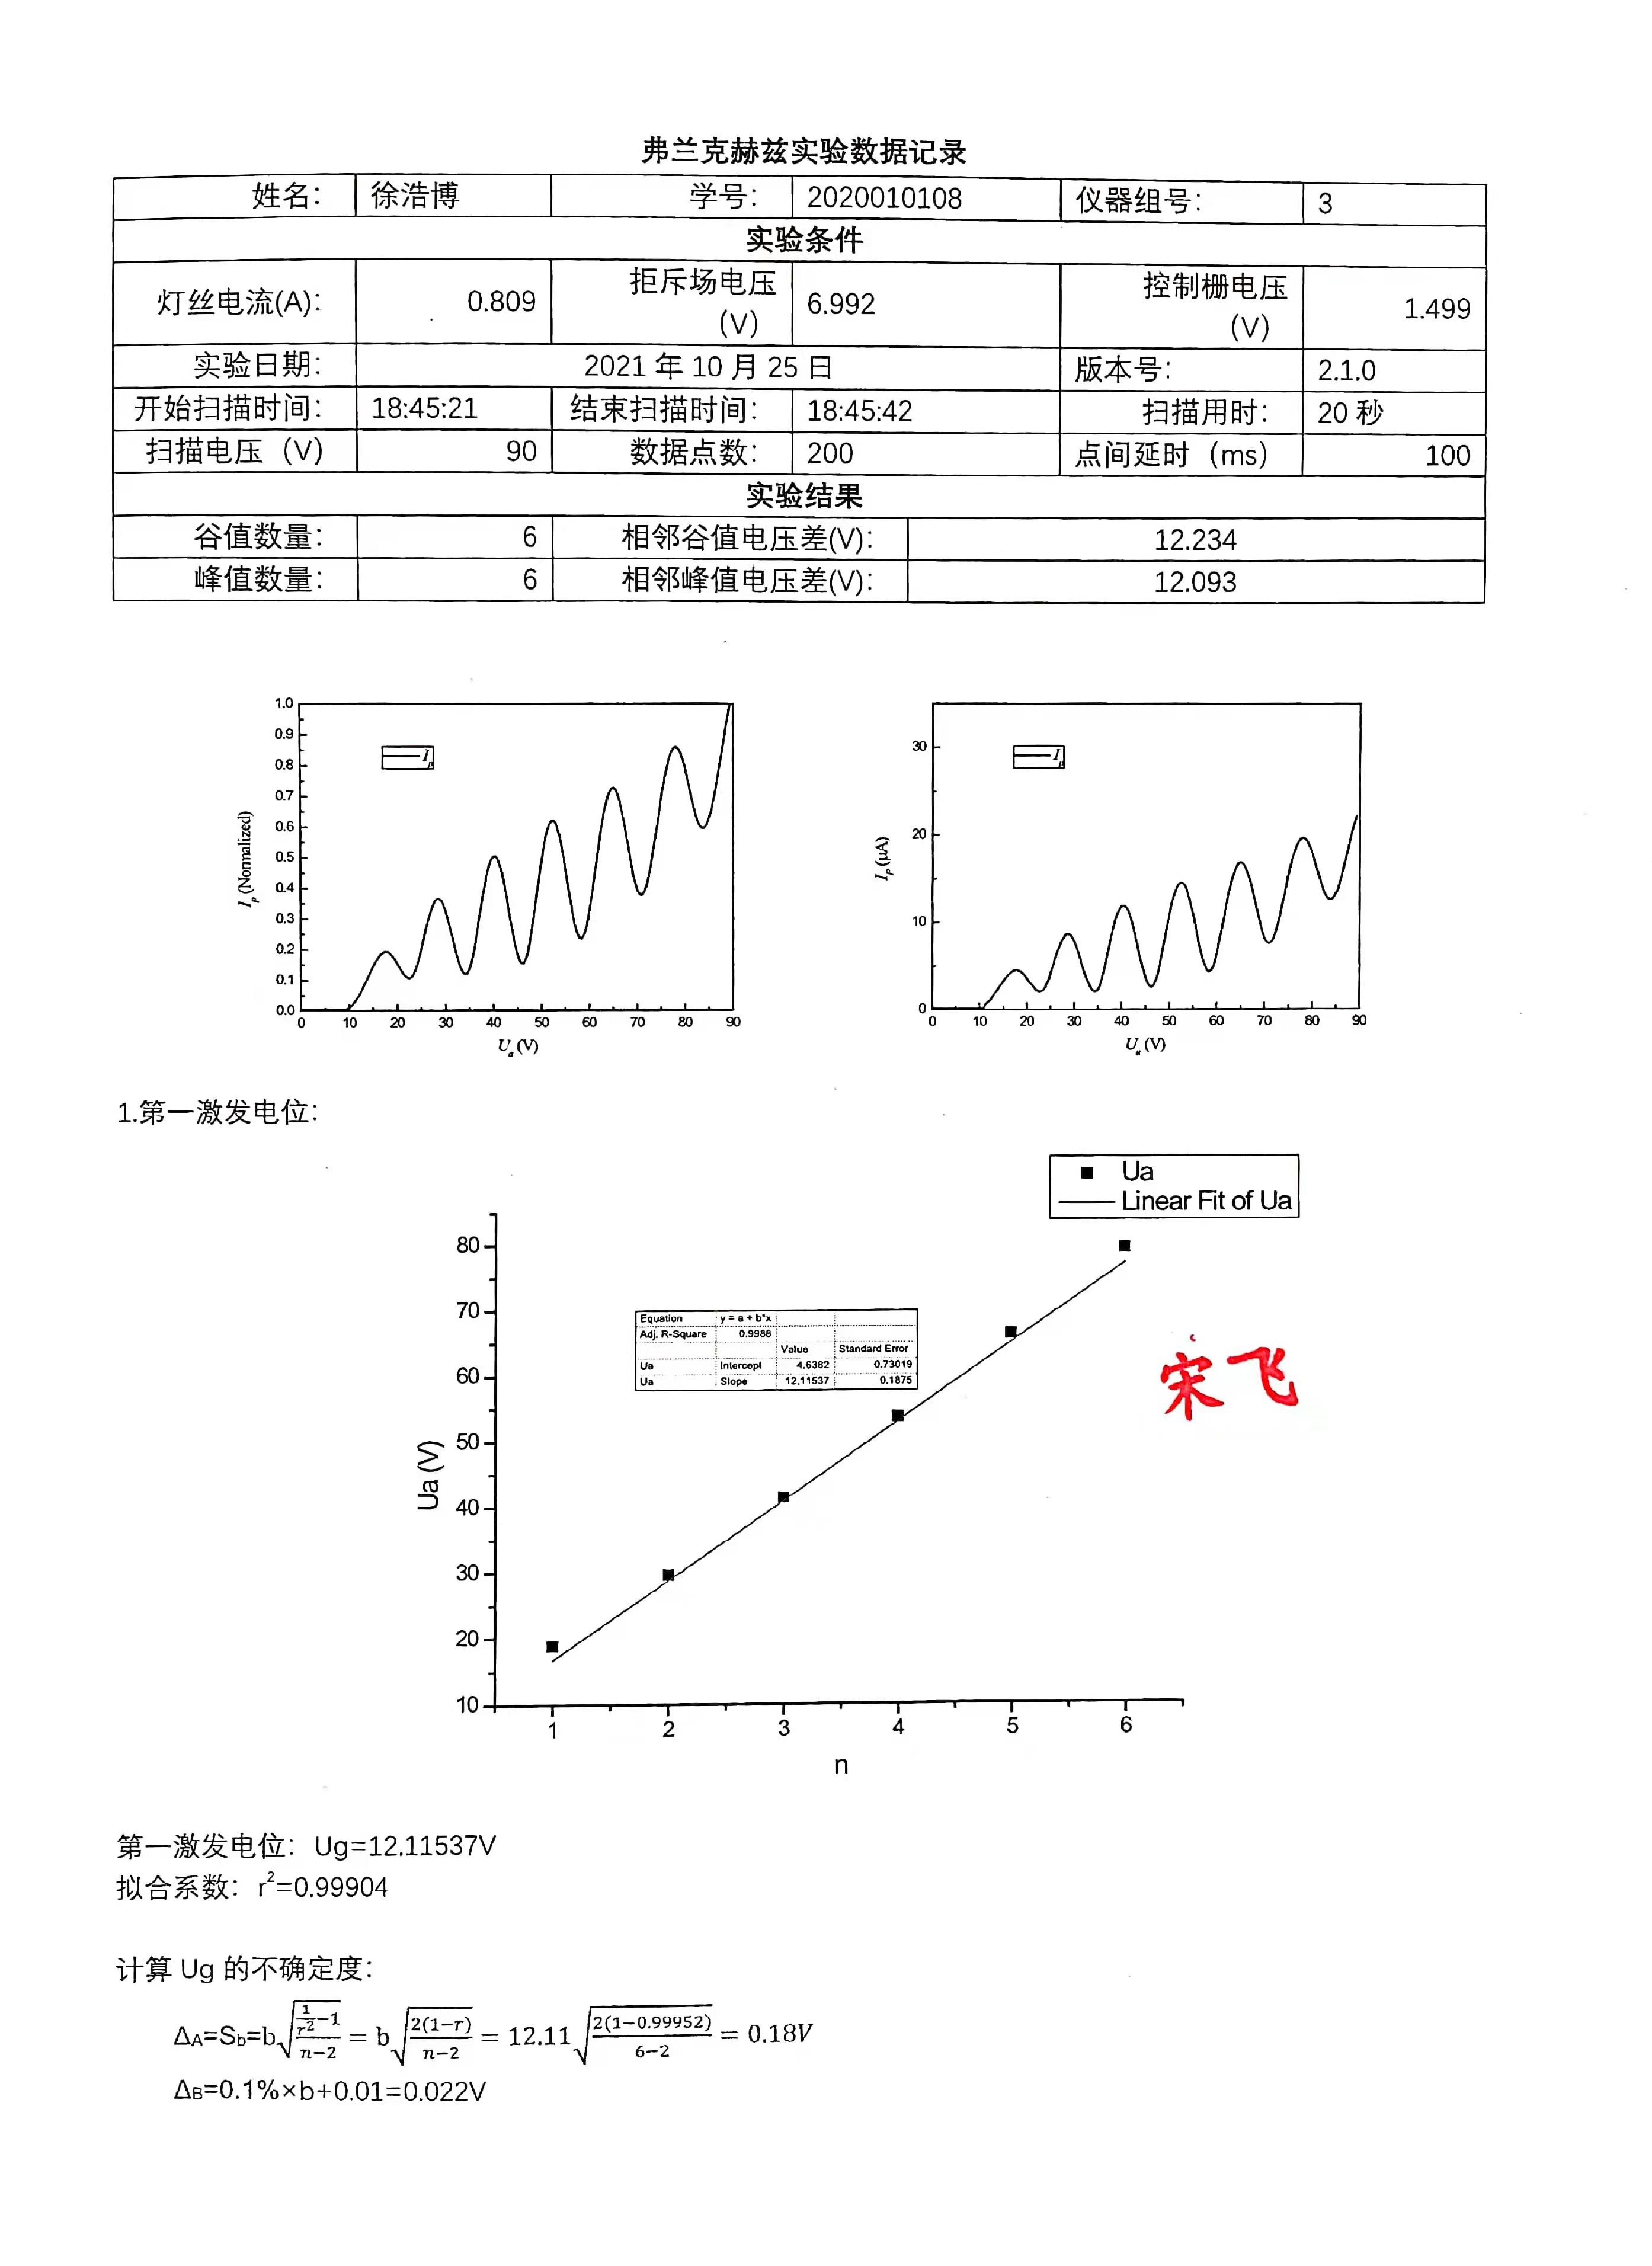
\includegraphics[scale=0.25]{data1.jpg}
    \end{center} \end{figure}


    \begin{figure}[H]\begin{center}
        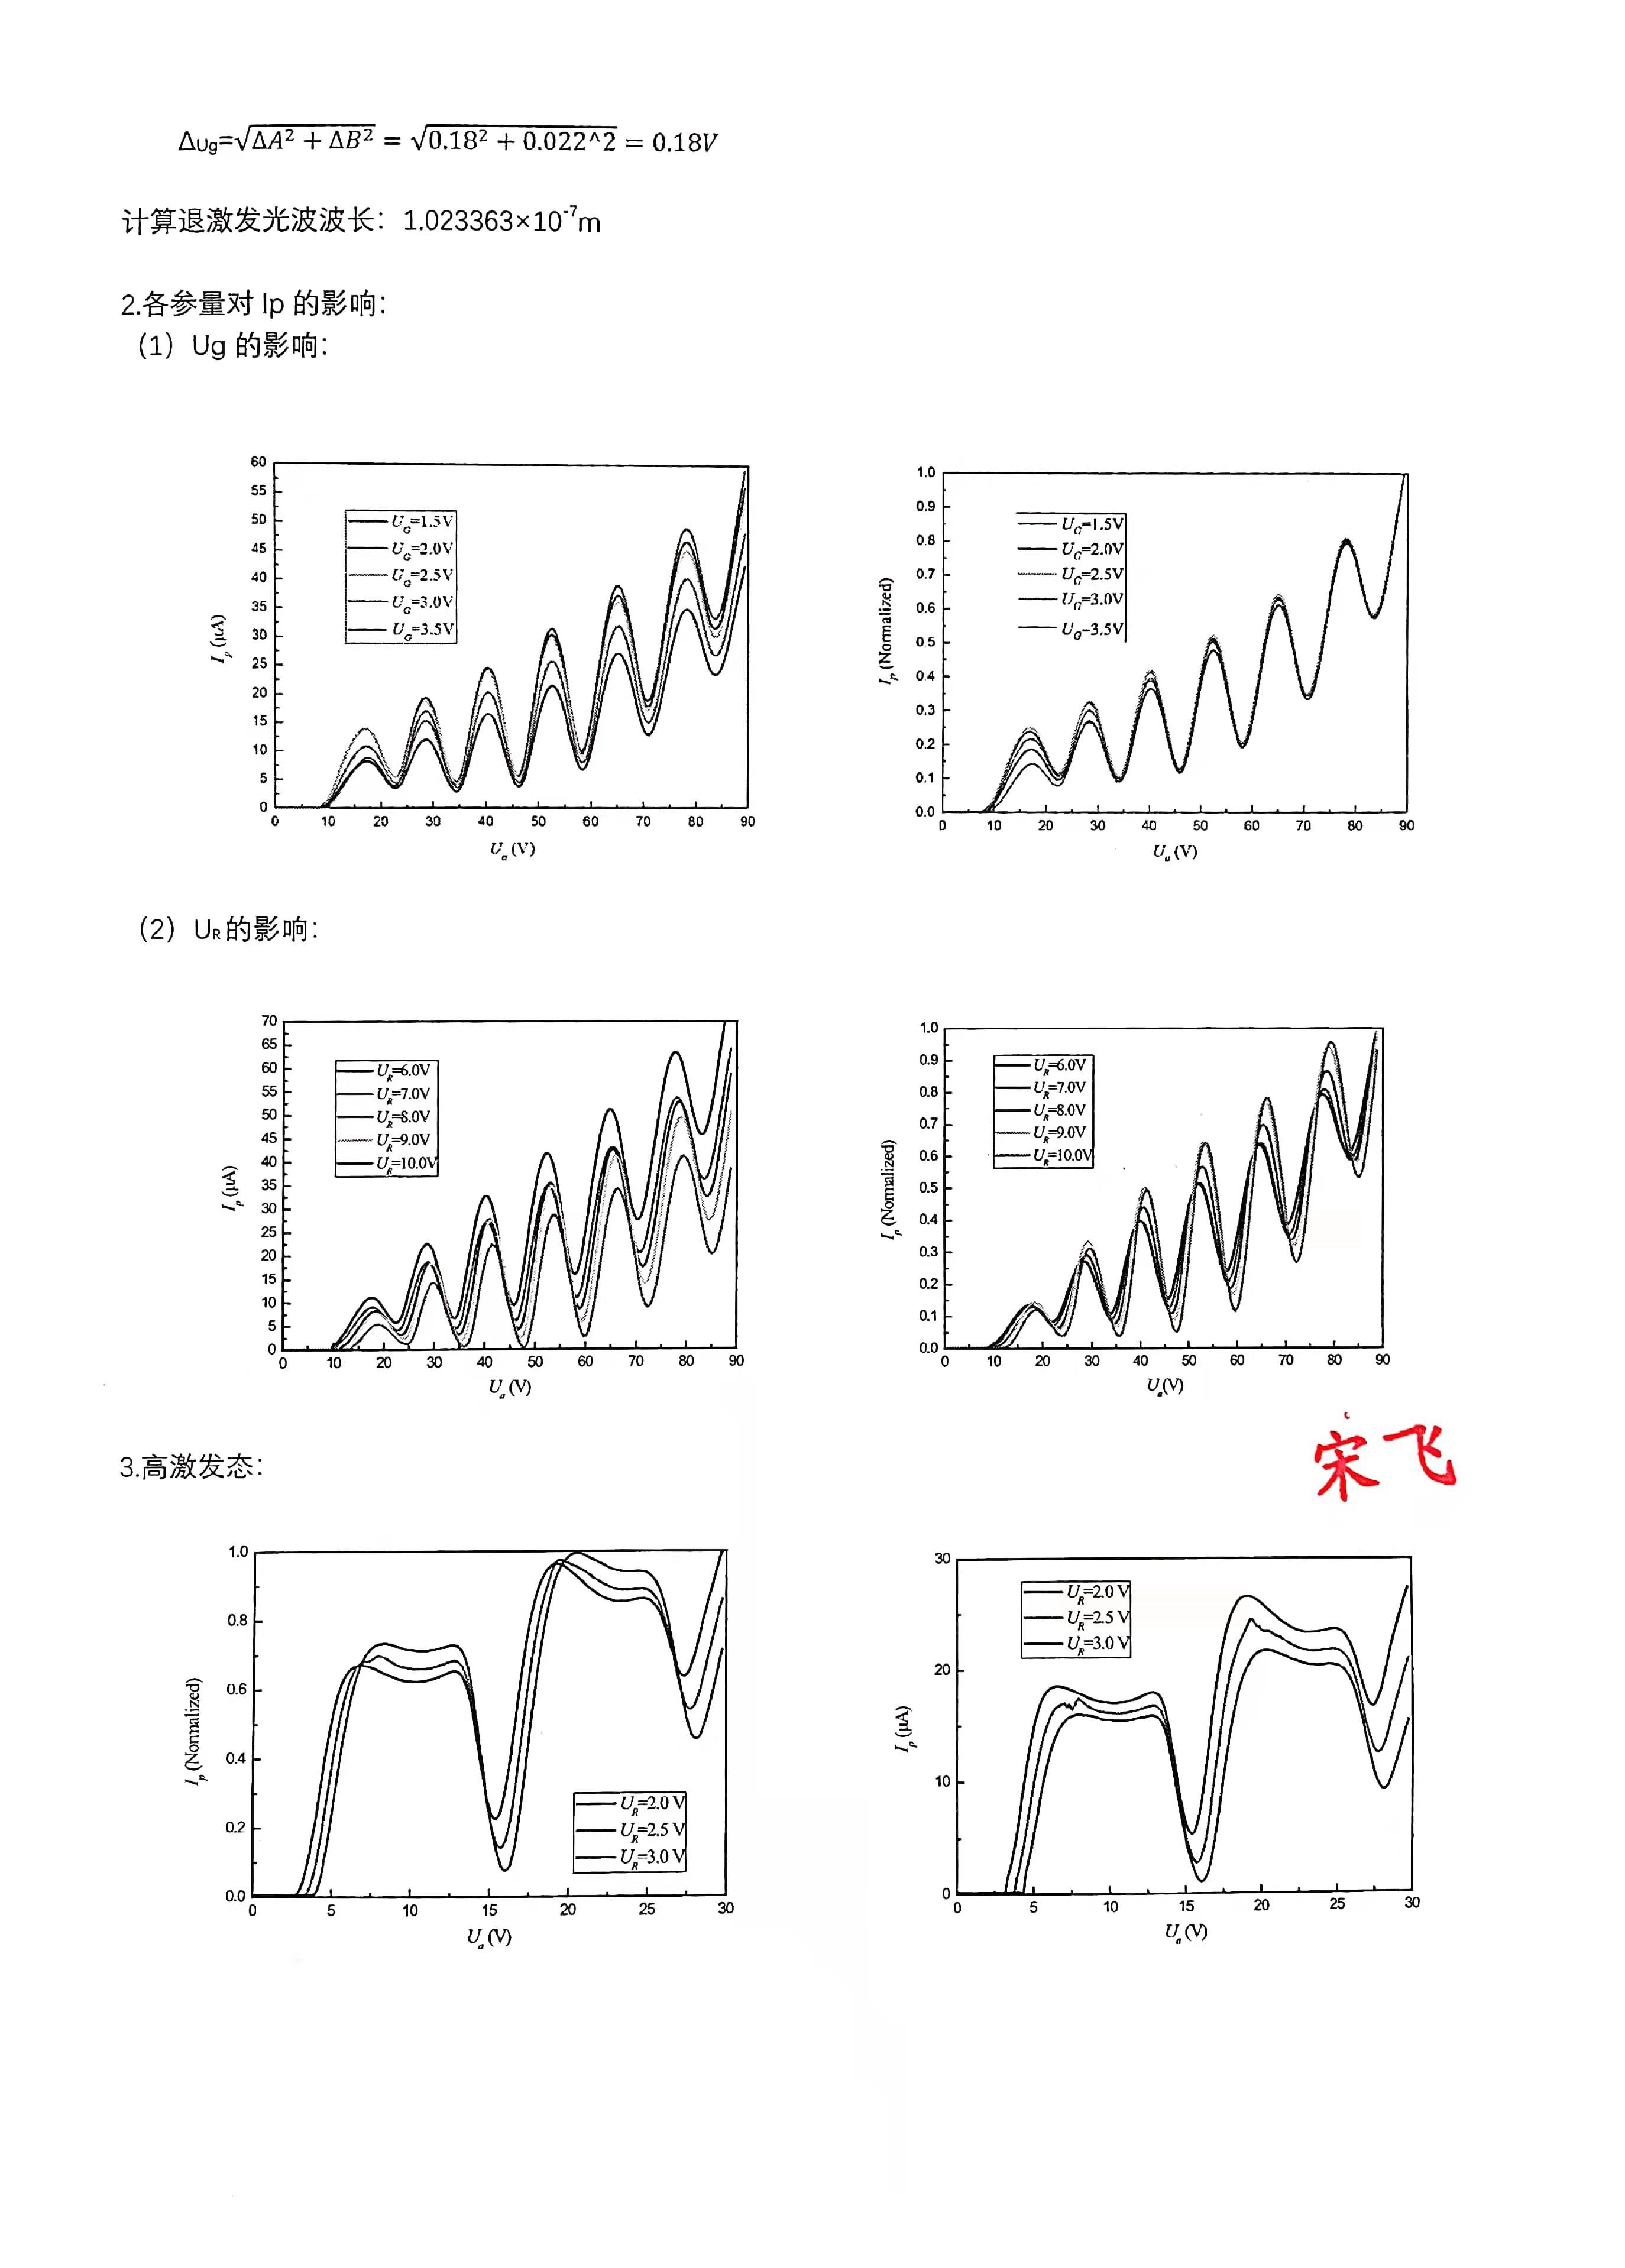
\includegraphics[scale=0.25]{data2.jpg}
    \end{center}  \end{figure}
    \vspace{-4em}
\section{参考文献}\quad\\
1. Energy Levels of Neutral Argon (Ar I). \href{https://physics.nist.gov/PhysRefData/Handbook/Tables/argontable5.htm}{https://physics.nist.gov/PhysRefData/Handbook/Tables/argontable5.htm}\\
2. Persistent Lines of Singly Ionized Argon (Ar II). \href{https://physics.nist.gov/PhysRefData/Handbook/Tables/argontable4.htm}{https://physics.nist.gov/PhysRefData/Handbook/Tables/argontable4.htm}\\
3. Strong Lines of Argon (Ar). \href{https://physics.nist.gov/PhysRefData/Handbook/Tables/argontable2.htm}{https://physics.nist.gov/PhysRefData/Handbook/Tables/argontable2.htm}
\end{document}

